\subsection{Implementation contract}
The archive contains a runnable proposed \path{fast/} source tree, a patch against the pinned baseline, the article sources, and independently runnable validation and benchmark drivers. The default recognizer and reducer are unchanged. The additions are:
\begin{itemize}
\item \path{fastunknot/graded_transfer.py}: quantum-shift tracking, binary special contractions, exact finite transfer, source-band pruning, eager and adaptive scan subclasses, and optional verification of all eight chain-contraction identities.
\item \path{fastunknot/twist/long_tail.py}: cap selection, interior-matrix extraction, exact compact homological profiles, coefficient queries, guarded materialization, and independently replayable dominant-run certificates.
\item \path{fastunknot/symbolic_braid.py}: signed-run structural certificates, an independent count verifier, exact homology fallback, and a CLI that accepts large hexadecimal exponents.
\end{itemize}

The two new scan modes are \code{graded} and \code{graded-adaptive}. They use the standard, minimum-fill, bitset scanner with one order race. They are not combined with the shared component scanner or the homological-window scanner: those classes allocate objects differently and do not yet carry the required quantum shifts. The ordinary \code{component} and \code{component-dense} coefficient composition adapters remain supported; the restriction concerns component sharing and window pruning. Unsupported combinations are rejected before an early topological filter can mask an invalid configuration. This is an interface restriction, not a claim that such combinations are mathematically impossible.

Resource failure returns \code{UNKNOWN} or raises the established resource exception at a lower-level API; it never becomes an unknot verdict. An optional ceiling on transfer objects falls back to ordinary exact scalar cancellation. The tail backend applies matrix budgets to the complex it actually constructs, retaining the original component count for recognition. Hexadecimal serialization is used for integers exceeding 4,096 bits; Python's decimal-conversion safeguards are not disabled.

\subsection{Validation beyond final ranks}
\newcommand{\FinalTestCount}{281}
\newcommand{\FinalTestSeconds}{52.285}

The baseline's 245 tests pass before modification. The integrated tree passes \FinalTestCount{} tests in \FinalTestSeconds{} seconds in the recorded run. The additional mathematical validation is deliberately stronger than agreement on a few named knot ranks:
\begin{itemize}
\item The transfer experiment uses 86 diagrams and 258 diagram/order presentations. All four tested modes agree in raw homological ranks; the three quantum-tracking modes also agree in quantum-resolved ranks. At 1,812 actual scan stages, the diagnostic verifier checks all eight identities in Theorem~\ref{thm:transfer}, including the contracting homotopy identity. The order presentations are not counted as distinct knots.
\item Seven dense valid graded controls retain a nonzero dotted differential between survivors. Eight perturbation-chain controls require correction terms of lengths one through eight. Other controls exercise paused/resumed reduction, a vanishing $x^2$ contribution beyond the source band, capacity fallback, and deadline propagation.
\item The tail tests make 240 complete degree-profile comparisons, 80 checks of the earlier $L+1$ rank threshold, 32 literal interior-matrix comparisons, and 24 comparisons with the independent crossing-cube builder. They include both signs, selected runs in different positions, links at the cap, original knots, and 20,001-bit exponents.
\item A separately written referee program builds 392 explicit macro complexes from 96 fixed contexts and sharpness cases. It checks $d^2=0$, Euler characteristic, the extracted repeated matrix, both thresholds, every homological coefficient, and the dominance bound. It does not call the new tail implementation to obtain the reference answer.
\item The succinct structural tests compare signed-graph counts with 180 expanded PD diagrams, compare applicable verdicts with exact Khovanov calculations in a separate 40-presentation sample, and exercise tampered certificates, malformed input, huge strand counts, huge exponents, and CLI exit semantics.
\item The repair-DAG verifier checks 380 explicit-path and closed-form fixtures, together with invalid-input rejection. These checks verify the combinatorial counting implementation, not the existence of such a dependency graph for knot exteriors.
\end{itemize}
The proofs establish the mathematical statements; the finite tests check the implementation and catch convention and indexing errors. There is no claim of machine-checked formalization in a proof assistant.

\subsection{Paired transfer measurements and a negative result}
All recorded timings use Python 3.12.14 on a shared Linux virtual environment. Seven seeded rounds shuffle the order of the baseline, an independent repetition of the same baseline (A/A), eager transfer, and adaptive transfer. Setup is excluded from these kernel or raw-scan timers; the actual reduction or scan is included. Small measurements are batched, and cyclic garbage collection is disabled only inside these timing regions. The complete sample arrays and inputs are retained.

Table~\ref{tab:gradedbench} reports median baseline time and median \emph{paired} time ratios. A ratio greater than one favors the proposed method; a ratio below one is a regression. A paired-ratio median need not equal the quotient of the two separately reported medians. The A/A column shows that the environment has material timing noise, so small changes should not be treated as reliable gains.

\begin{table}[htbp]
\centering\small
\begin{tabular}{@{}lrrrr@{}}
\toprule
Input & Baseline (ms) & Eager ratio & Adaptive ratio & A/A \\
\midrule
Hard unknot, 8 crossings & 1.597 & 0.609 & 0.913 & 0.935 \\
Conway & 8.115 & 0.559 & 0.846 & 0.801 \\
Kinoshita--Terasaka & 11.179 & 0.673 & 1.215 & 1.313 \\
Unknot braid, 40 crossings & 1.653 & 0.476 & 0.783 & 0.903 \\
Stress braid, 36 crossings & 657.597 & 0.263 & 0.989 & 1.057 \\
Algebra: 66 objects & 0.495 & 0.758 & 0.611 & 0.774 \\
Algebra: 130 objects & 3.378 & 1.995 & 1.532 & 0.996 \\
Algebra: 258 objects & 37.729 & 6.521 & 4.057 & 0.899 \\
Algebra: 514 objects & 398.976 & 15.308 & 11.760 & 0.900 \\
\bottomrule
\end{tabular}

\caption{Transfer measurements. The last four rows are valid algebraic controls, not diagram inputs; each has two survivors and a nonzero minimal differential. Ratios are baseline time divided by the indicated arm's time.}
\label{tab:gradedbench}
\end{table}

The 258-object and 514-object controls show the intended regime: many scalar contractible objects, few survivors, and substantial sparse Schur work. Eager transfer attains paired median gains of approximately $6.52$ and $15.31$; the adaptive version attains $4.06$ and $11.76$. This is evidence that the new primitive can be useful, not evidence that a typical knot scan has this structure.

On the ordinary diagram inputs eager transfer loses, including an approximately $3.8$-fold paired slowdown on the 36-crossing stress input. The adaptive variant makes no transfer calls on these five ordinary scans: its work is the existing sparse path plus tracking and dispatch overhead. The slight apparent gains or losses there do not establish an ordinary-diagram improvement, especially given the A/A variation. Keeping the new modes optional is therefore part of the result. Changing the default on the basis of the algebraic controls would be unsupported.

\subsection{Finite-tail homology measurements}
The long-tail experiment uses sixteen configurations, both signs, and seven seeded paired rounds with an independent ordinary-macro A/A arm. These timers include complex construction and exact homology; they exclude input construction. Every timed answer is compared in every homological degree. The cap arm also checks the interior matrix square. The reported kernel hash matches the bundled implementation. Only portable import and output paths differ between the measured and distributed benchmark drivers; the supplied patch records those changes.

\begin{table}[htbp]
\centering\small
\begin{tabular}{@{}rrrrrr@{}}
\toprule
Strands & Exponent & Original basis & Cap basis & Speedup & A/A \\
\midrule
4 & +801 & 142,011 & 1,650 & 45.25 & 0.862 \\
4 & $-801$ & 142,011 & 1,650 & 45.19 & 0.827 \\
5 & +801 & 358,941 & 4,917 & 34.42 & 1.066 \\
5 & $-801$ & 358,941 & 4,917 & 34.25 & 0.968 \\
\bottomrule
\end{tabular}

\caption{Raw homology at signed exponent magnitude 801. Each context has interior Betti number $\nu=3$. These inputs are already decided by the structural recognition filters.}
\label{tab:tailbench}
\end{table}

For the four-strand context, the cap basis remains 1,650 as the original basis grows from 9,261 at $m=51$ to 142,011 at $m=801$. The five-strand context uses 4,917 cap basis elements, versus 358,941 original ones at $m=801$. The paired gains at $801$ range from approximately $34.25$ to $45.25$. Across all sixteen configurations the A/A medians range from $0.827$ to $1.194$. Figure~\ref{fig:tailtime} shows the positive-run timings with their observed interquartile ranges; it is a sample of the expected constant-cap behavior, not a fit establishing the asymptotic theorem.

\begin{figure}[htbp]
\centering
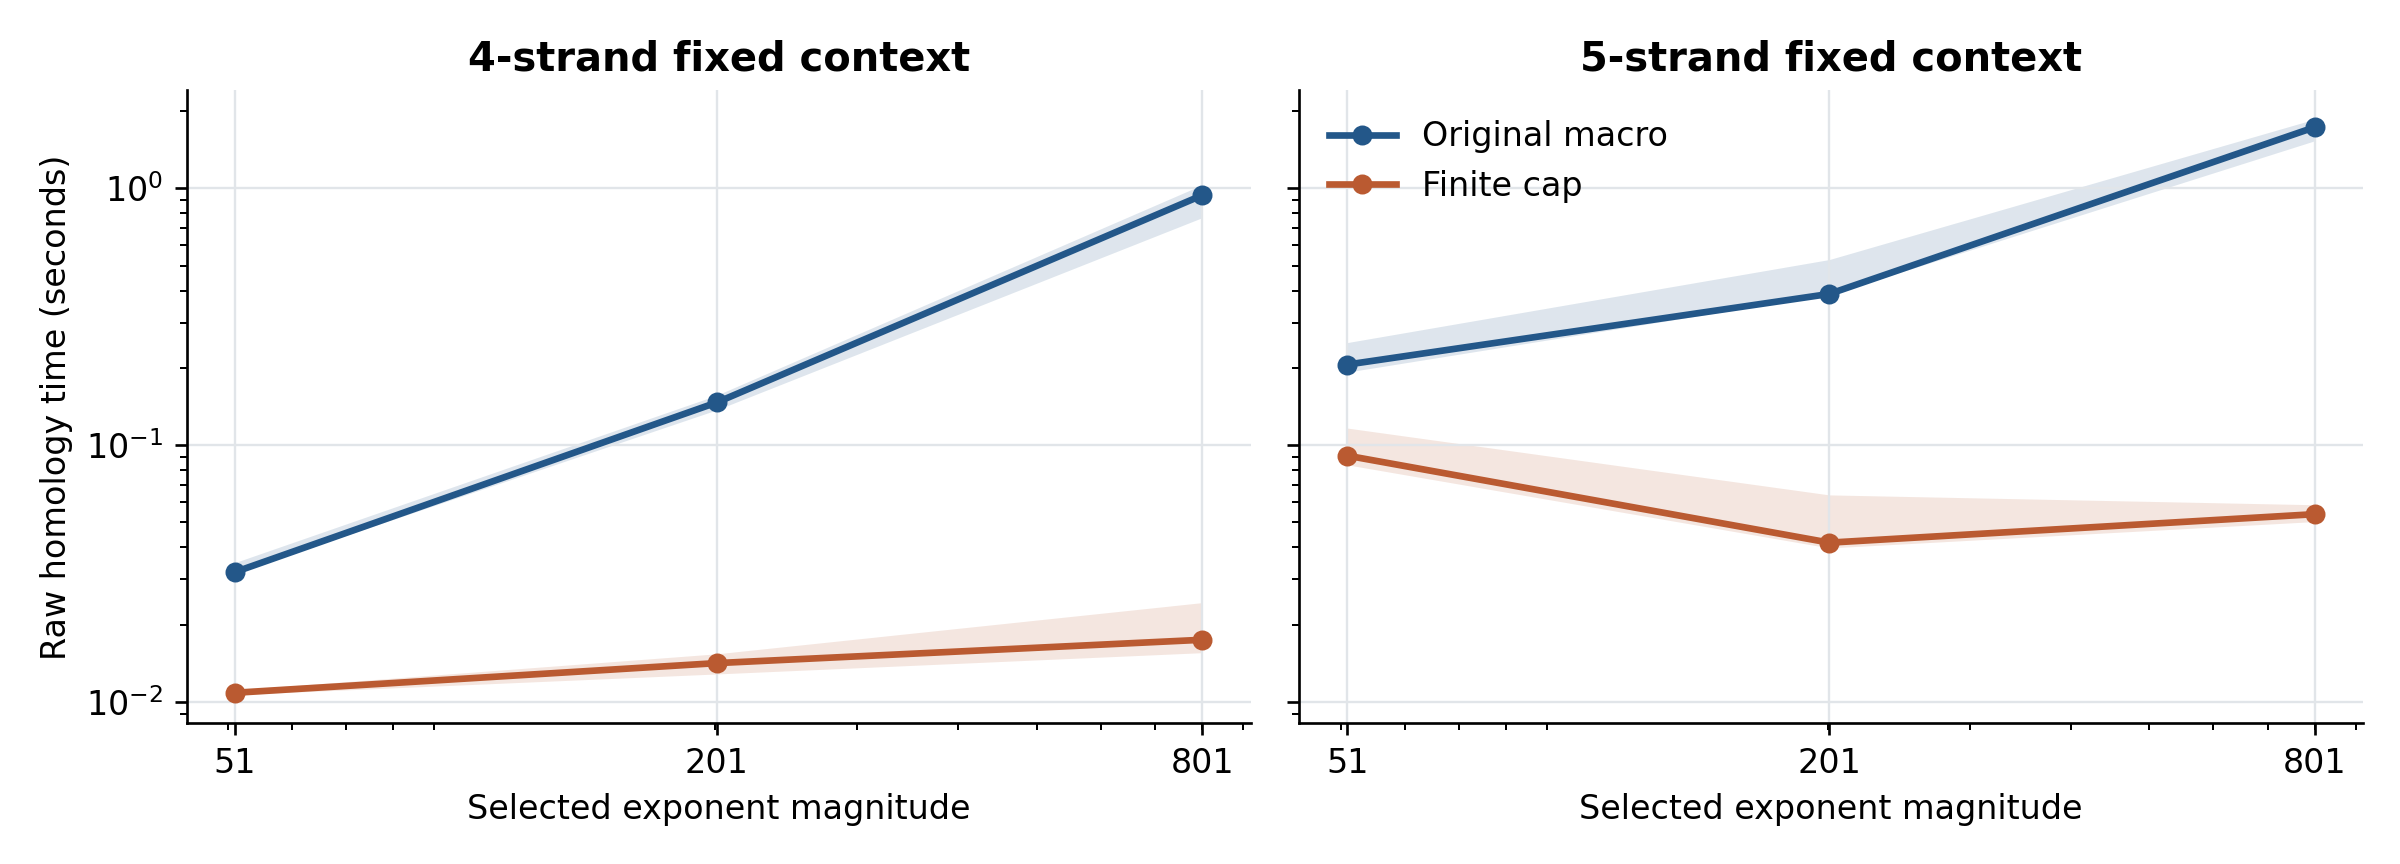
\includegraphics[width=\textwidth]{figures/tail_timings.png}
\caption{Median raw homology time for fixed contexts; shading spans the first and third quartiles of seven samples. The original macro construction grows with the selected exponent; the cap calculation uses the same finite complex. Both axes are logarithmic.}
\label{fig:tailtime}
\end{figure}

A more informative exact-size example uses
\[
 \sigma_2^{-1}\sigma_1\sigma_2\sigma_3^M
 \sigma_2^{-1}\sigma_1\sigma_3^{-1},\qquad M=10^{100}+1.
\]
Here $L=6$, the cap is eight, and $\nu=3$. The result has total rank
\[
 3M-2=3\cdot10^{100}+1,
\]
represented by eleven exceptional points and one constant interval, using 1,650 basis elements. The recorded calculation takes about $0.035$ seconds including $d^2$ and $A^2$ checks. This time is illustrative; the exact finite representation is the substantive result. The cap is a two-component link while the original closure is a knot, demonstrating why the component check must refer to the original exponent.

All these long-tail knots are structurally easy for the maintained recognizer. The finite-cap result accelerates their \emph{requested exact homology}; it is not a measured improvement on hard unknot decisions. Report 14's earlier interval experiment imposed a common matching and common square-zero coefficient on an entire connected differential summand. The present argument instead uses a full matrix $A$ containing arbitrary fixed-context state maps, and the examples above are actual braid closures. The wider applicability of this closed-complex calculation does not make it a relative-boundary replacement.

\subsection{Direct structural evaluation on run input}
The supplied balanced example is the five-strand closure
\[
 \sigma_1^M\sigma_2^{-M}\sigma_3^M\sigma_4^{-M},\qquad M=10^{100}+1.
\]
Its writhe is zero and none of its four runs dominates the rest. The signed Seifert graph is homogeneous, with canonical genus $2M-2=2\cdot10^{100}$. The succinct front end certifies nontriviality directly. This illustrates an improvement in the representation accepted by the implementation, using an existing topological criterion.
A focused interface benchmark uses this same four-run family with magnitudes
101, 1,001, and 10,001. Each arm starts with the identical already parsed run
tuple. The expanded arm includes letter expansion, fresh PD construction and
validation, and the maintained Seifert certificate; the direct arm evaluates
the signed-run certificate. The latter batches 100 fresh calls per sample.
Seven shuffled paired rounds include an expanded A/A arm. Every common
certificate field agrees, and all 2,100 direct certificates pass independent
verification outside the timers.
\begin{table}[htbp]
\centering\small
\begin{tabular}{@{}rrrrr@{}}
\toprule
Magnitude & Crossings & Expanded (ms) & Direct ($\mu$s) & A/A \\
\midrule
101 & 404 & 4.787 & 5.971 & 1.053 \\
1,001 & 4,004 & 48.083 & 5.039 & 1.039 \\
10,001 & 40,004 & 484.068 & 4.482 & 0.958 \\
\bottomrule
\end{tabular}

\caption{Structural certificate evaluation from the same run input. Note the
different time units. These timings include the representation conversion
required by the expanded route and do not measure the full recognition portfolio.}
\label{tab:structural}
\end{table}
The direct call takes roughly five microseconds at these sizes while the
expanded route grows from about five to 484 milliseconds. The input has four
runs throughout; this measures the work avoided by the representation change.
The shared environment included a concurrent regression run, recorded in the
raw JSON. The exact timings and especially very large ratios should therefore
be read as interface measurements, not transferable hardware constants.


\subsection{Reproduction and integration}
Run the following from the archive root to execute the complete integrated suite and the separate mathematical checks:
\begin{lstlisting}[language=bash]
python tools/verify_all.py
\end{lstlisting}
The benchmark commands are separate, so reproducing correctness does not silently replace the delivered measurements. The top-level README gives all commands, input conventions, evidence paths, and the patch workflow. For example:
\begin{lstlisting}[language=bash]
cd implementation/fast
python -m fastunknot khovanov examples/conway.json \
  --reduction graded-adaptive
python -m fastunknot.symbolic_braid \
  ../../examples/four_strand_tail.json --mode homology --check-d2
python -m fastunknot.symbolic_braid \
  ../../examples/balanced_four_runs.json --mode certificate
\end{lstlisting}
The article rebuild script invokes \code{pdflatex} until references stabilize, using the delivered tables and figure. A separate evidence-refresh script can regenerate them from a new run's JSON. The patch is checked against the exact baseline and can be reviewed before application; the runnable proposed source tree is included for inspection without patching a working checkout.

